\newpage
\section{Экспериментальная часть}
Экспериментальная методика, использованная в данной работе, предусматривает несколько основных этапов: 
приготовление газовой смеси необходимой концентрации; получение твёрдого образца путём осаждения газа на холодную подложку криостата; 
облучение рентгеновским излучением; запись ИК-спектров.
\subsection{Используемые вещества}
В качестве матриц применяли благородные газы Ne (99.996\%), Ar (99.998\%), Kr (99.99\%), Xe (99.9996\%) без дополнительной очистки. Бензол (ХЧ, Lachema, Chemapol), бензол-$d_6$ (99.6 атом \% D, Sigma-Aldrich Chemie GmbH) использованы без дополнительной очистки.
\subsection{Приготовление газовых смесей}
Приготовление газовых смесей\footnote{вед. инж. И. В. Тюльпина} осуществляли с помощью установки, 
изображённой на рисунке~\ref{gas}. Мольное соотношение компонентов смеси ($n_1/n_2$) определяли в приближении идеального газа: $n_1/n_2=p_1V_1/p_2V_2$, 
где $V_1$ и $V_2$~--- объёмы, заполняемые газами; $p_1$ и $p_2$~--- давления каждого газа. Установку предварительно вакуумировали до остаточного давления 0.1~Па, 
малую калибровочную ёмкость заполняли исследуемым газом (паром) до необходимого давления и вымораживали в газовую ампулу-приёмник. 
Большую калибровочную ёмкость использовали для отбора матричного газа, который затем также вымораживали в ампулу-приёмник.
\newpage
\begin{figure}[H]
\center{\includegraphics[width=0.5\linewidth]{vu_.pdf}}
\caption{Схема установки для приготовления газовых смесей. 1~--- ампула с исследуемым веществом; 2~--- малая ёмкость с калиброванным объёмом; 3~--- большая ёмкость с калиброванным объёмом; 4~--- ампула для готовой газовой смеси; 5~--- манометр; 6~--- подключение вакуумного поста; 7~--- подключение баллона с матричным газом.}
\label{gas}
\end{figure}
\subsection{Криостат}
В настоящей работе применяли метод ИК-спектроскопии в условиях матричной изоляции. 
Методика экспериментов основана на использовании гелиевого криостата оригинальной конструкции, разработанного в лаборатории химии высоких энергий 
Химического факультета МГУ, на основе серийного криорефрижератора замкнутого цикла Sumimoto Heavy Ind. SRDK-101D-A11C. 
Принципиальная схема криостата изображена на рисунке~\ref{IR}.
Нагнетаемый компрессором гелий расширяется в ступенях рефрижератора, охлаждая криостат. 
Температуру измеряли при помощи термопары медь/медь-железо, обладающей высокой чувствительностью в области гелиевых температур. 
Для регулировки температуры использовали два нагревателя, подключённые к источнику постоянного тока и цифровой контроллер t-Stat. 
Заданная температура поддерживалась с точностью 0.5~К. Измерение температуры осуществляли при помощи контроллеров t-Stat и LakeShore. 
Для измерения давления использовали термопарные лампы ПМТ-2 с вакууметрами Мерадат. Давление внутри криостата не превышало 10$^{-4}$~кПа. 
Криостат для исследований методом ИК-спектроскопии оснащён подложкой для образца, изготовленной из KBr, окошками из КРС для записи ИК-спектров, 
окошком из алюминиевой фольги для облучения рентгеновским излучением, кварцевыми окошками для фотолиза видимым и ближним УФ-излучением.
\begin{figure}[H]
\center{\includegraphics[width=0.6\linewidth]{cryo_numb.pdf}}
\caption{Схема гелиевого криостата замкнутого цикла для проведения исследований. 1 и 2~--- вход и выход компрессора со сжатым гелием; 3~--- подключение вакуумной линии и установки осаждения; 4~--- подключение термоконтроллера; 5~--- первая ступень охлаждения (300--44~K); 6~--- капилляр для осаждения образца; 7~--- вторая ступень охлаждения (44--6~K); 8~--- оптическое окно из КРС-5; 9~--- нагреватель~2; 10~--- подложка из KBr для осаждения образца, держатель, термопара Cu/Fe-Cu, нагреватель~1; 11~--- направление луча ИК-спектрометра; 12~--- защитный экран от теплового излучения; 13~--- вращающийся вакуумный кожух.}
\label{IR}
\end{figure}
\subsection{Осаждение образца и определение толщины слоя}
Для приготовления образца газовую смесь медленно осаждали на охлаждённую подложку криостата, используемая установка изображена на рисунке~\ref{dep}. 
Температуру подложки устанавливали до начала осаждения таким образом, чтобы получить образец с наилучшими оптическими свойствами и близким к равномерному 
распределением исследуемых молекул внутри матрицы. Типичные температуры, использованные для получения матриц в данной работе, составляют 
15--18~K для Ar, 21--25~K для Kr и 25--30~K для Xe. Газовую смесь пропускали через вентиль тонкой регулировки, который позволяет регулировать давление 
внутри коммуникации в процессе осаждения. Типичное время напыления образца составляет 1--1.5~часа.
\begin{figure}[H]
\center{\includegraphics[width=0.6\linewidth]{dep.png}}
\caption{Схема установки подачи газовой смеси в криостат}
\label{dep}
\end{figure}
Толщину образца в ИК-криостате определяли по интерференции, видимой в ИК-спектре (Рисунок~\ref{inter}). 
Интерференция наблюдается при отражении волны от поверхностей раздела фаз: воздух/образец и образец/материал подложки (KBr). 
Отражение происходит при значительном различии коэффициентов преломления двух фаз. Коэффициент преломления воздуха равен 1, 
для  аргона, криптона и ксенона его значения составляют 1.2, 1.3 и 1.4, соответственно~\cite{Sinnock1980}, 
для KBr~--- 1.55. Формула для расчёта толщины слоя: $d = 1/(2n(\nu_1-\nu_2))$, где $d$~--- толщина, $n$~--- коэффициент преломления
матрицы, $(\nu_1-\nu_2)$~--- длина периода интерференции, наблюдаемая в спектре. Толщины образцов в проведённых экспериментах составляют 
120--200~мкм для неоновой матрицы и 70--120~мкм в случае аргона, криптона и ксенона.
\begin{figure}[H]
\center{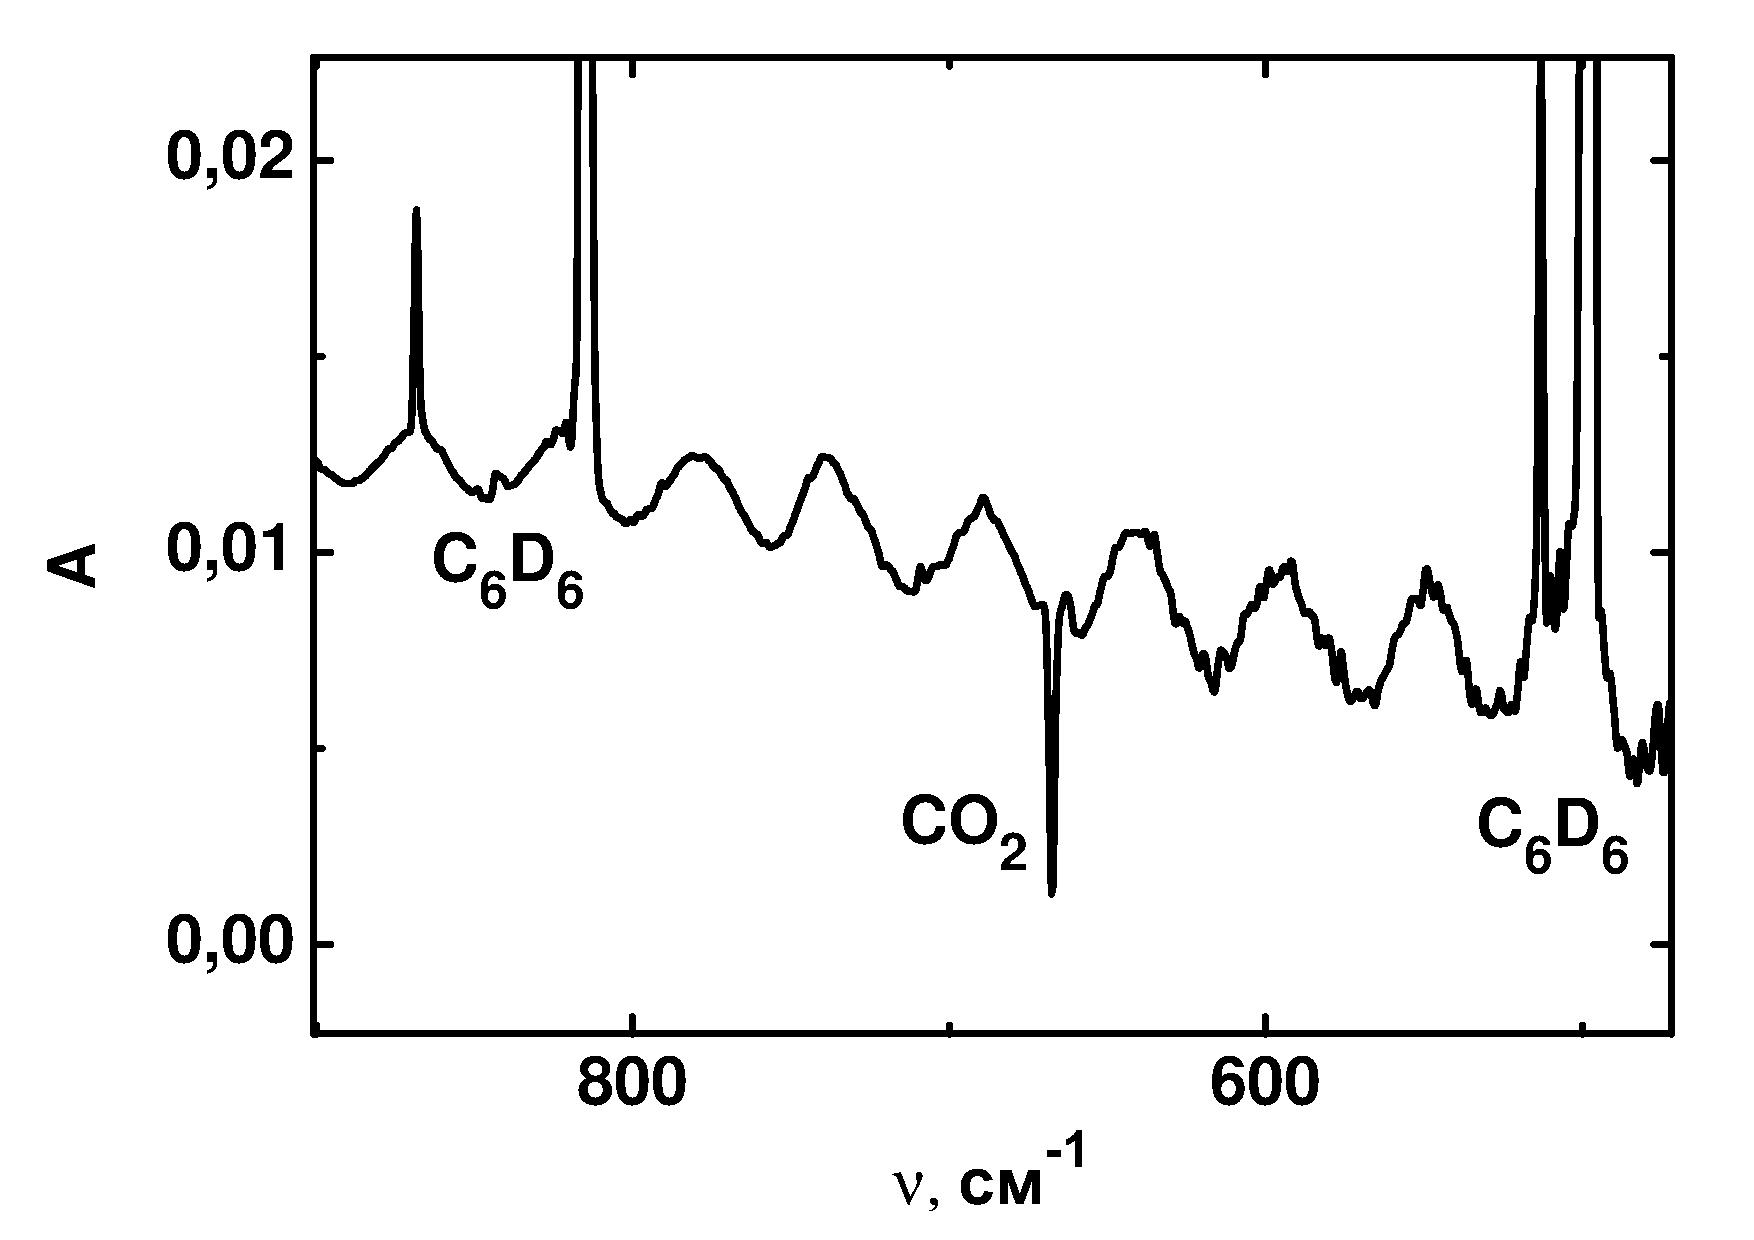
\includegraphics[width=0.8\linewidth]{inter.pdf}}
\caption{Интерференционная картина, наблюдаемая в ИК-спектре осаждённого образца C$_6$D$_6$/Ar}
\label{inter}
\end{figure}
\subsection{Радиолиз и фотолиз}
Осаждённый образец охлаждали до минимальной температуры (5--7~K в зависимости от особенностей сборки криостата) 
и подвергали действию излучения рентгеновской трубки 5-БХВ6-W с вольфрамовым анодом с максимальной энергией кванта около 32~кэВ 
(эффективная энергия составляет примерно 20~кэВ).
Для оценки мощности дозы использовался ферросульфатный дозиметр (дозиметр Фрикке), радиационно-химический выход ионов Fe$^{3+}$
 в котором равен 14.4~иона/100~эВ при эффективной энергии рентгеновского излучения 20~кэВ \cite{Pikaev}. 
 В геометрии облучения образца в ИК-криостате мощность дозы для дозиметрического раствора составила 0.72 Гр/с.
 Полученную величину мощности дозы пересчитывали с учётом массовых коэффициентов поглощения среды для осаждённых плёнок инертных газов 
 по формуле:
$I(\mathrm{Ng}) = \frac{\mu(\mathrm{Ng})\cdot I(\mathrm{H_2O})}{\mu(\mathrm{H_2O})}$, где $I(\mathrm{Ng})$ и $I(\mathrm{H_2O})$~--- мощности дозы для благородного газа и дозиметрического раствора, соответственно, $\mu(\mathrm{Ng})$ и $\mu(\mathrm{H_2O})$~--- массовые коэффициенты поглощения для благородного газа и дозиметрического раствора (последний считается равным коэффициенту для воды). Массовые коэффициенты поглощения и полученные значения мощности дозы представлены в таблице \ref{dose}.
\begin{table}[H]
\caption{Массовые коэффициенты поглощения \cite{xray} и мощности поглощённой дозы в матрицах инертных газов}
\label{dose}
\begin{center}
\begin{tabular}{c|cccc}
 & H$_2$O & Ar & Kr & Xe \\
 \hline
$\mu$, см$^2$/г & 0.55 & 8.1 & 35 & 25 \\
$I$, Гр/с & 0.72 & 11 & 47 & 33 \\
\end{tabular}
\end{center}
\end{table}

Следует, однако, отметить, что приведённые дозиметрические данные (как и рассчитанные на их основе величины радиационно-химических выходов) 
носят оценочный характер, поскольку спектр излучения имеет непрерывный характер, а массовые коэффициенты поглощения очень сильно (и притом немонотонно)
 зависят от энергии фотона в этой области. Кроме того, даже при толщинах осаждённого слоя до 100~мкм в криптоне и ксеноне возникает заметная 
 неоднородность распределения дозы по толщине образца (по этой причине использование более толстых слоёв нецелесообразно).

Фотолиз в видимой и ближней УФ областях проводили при помощи узкополосных диодных источников через кварцевые окошки криостата. 
Длины волн максимумов испускания использованных диодов приведены в таблице \ref{diod}.

Фотолиз в УФ области проводили при помощи ртутных газоразрядных ламп низкого и среднего давлений
ОУФ-6  и ОУФв\nobreakdash-02 <<Солнышко>>.

\begin{table}[H]
\caption{Длины волн максимумов испускания использованных диодов}
\label{diod}
\begin{center}
\begin{tabular}{lc}
Диод & Длина волны, нм \\
\hline
Красный & 625 \\
Оранжевый & 605 \\
Жёлтый & 590 \\
Зелёный & 525 \\
Синий & 460 \\
УФ & 400 \\
\end{tabular}
\end{center}
\end{table}

\subsection{Регистрация ИК-спектров}
ИК-спектры регистрировали с помощью Фурье-ИК спектрометра Bruker Tenzor II, снабжённого охлаждаемым жидким азотом полупроводниковым детектором MCT.
Спектры регистрировали в диапазоне волновых чисел 7500--400~см$^{-1}$ с разрешением  
1~см$^{-1}$, что было достаточно для целей эксперимента, и проводили усреднение по 144~сканированиям. 
Управление спектрометром осуществляли при помощи персонального компьютера с использованием программного обеспечения OPUS. 
Все спектры регистрировали при минимальной температуре.
\subsection{Квантово-химические расчёты}
Квантово-химические расчёты выполнены Сосулиным И.С. с использованием метода DFT(PBE). Данный функционал обеспечивает удовлетворительное описание энергетических и геометрических свойств для довольно обширного круга соединений при небольшой вычислительной стоимости \cite{Ernzerhof1999}. Кроме того, показано \cite{Furera2006, POPOV}, что расчёты на уровне PBE/TZ2P с хорошей точностью воспроизводят ИК спектры ароматических и полиароматических соединений. Для проведения расчетов применялся валентный корреляционно-согласованный базисный набор, L2\_3 
\cite{Laikov2005}. 
Базис L2\_3 является аналогом широко известного набора cc-pVTZ 
\cite{Kendall1992}, но отличаются от них большим числом элементарных гауссовых функций. Схема сжатия базисных наборов L2\_3, cc-pVTZ представлена в Приложении А. Данный базисный набор обеспечивает лучшее описание совокупности свойств молекулярных систем, чем аналогичный базис Даннинга. В то же время показано, что при больших n результаты расчётов в базисах Ln\_3 и соответствующих cc-pVXZ базисах сходятся друг к другу \cite{Laikov2005}. Точность самосогласования электронной задачи составляла 10$^{-10}$ а.е., геометрии оптимизировались до нормы градиента 10$^{-6}$ а.е. На оптимизированных геометриях решалась колебательная задача в гармоническом приближении с определением частот колебаний, ИК-интенсивностей и энергии нулевого колебательного уровня. Существование минимума на поверхности потенциальной энергии подтверждалось отсутствием мнимых частот колебаний у данной структуры. Для проведения расчётов использовался пакет программ PRIRODA, любезно предоставленный Д. Н. Лайковым \cite{Laikov}. Проведённые нами неэмпирические расчёты не учитывают влияния среды, то есть формально относятся к молекулам в вакууме (или газовой фазе), что может приводить к некоторому  расхождению экспериментальных и расчётных частот.











